\documentclass[11pt]{article}

\usepackage[margin=1in]{geometry}
\usepackage{graphicx}
\usepackage{hyperref}
\usepackage{xcolor}
\usepackage{listings}
\usepackage{cite}

\lstset{
  basicstyle=\ttfamily\small,
  breaklines=true,
  columns=fullflexible,
  frame=single,
  rulecolor=\color{black!20},
  keywordstyle=\color{blue!60!black},
  commentstyle=\color{black!60},
  stringstyle=\color{green!40!black},
  showstringspaces=false
}

\title{COMP7940 Cloud Computing\\Lab 3: Consuming External Service -- ChatGPT}
\author{
  Name: ZHAO Zhan \\
  Student ID: 25482351 \\
  GitHub: @Extious
}
\date{\today}

\begin{document}
\maketitle

\section*{1. Architecture of the Chatbot System}

The chatbot system consists of the following components:

\begin{itemize}
  \item \textbf{Telegram Bot Client}: Runs on the user's local machine (or server). It uses \texttt{python-telegram-bot}~\cite{python-telegram-bot,telegram-bot-api} to connect to Telegram's API and receive/send messages via long polling.
  \item \textbf{chatbot.py}: The main entry point running locally. It loads \texttt{config.ini}, creates a \texttt{ChatGPT} client, registers message handlers, and starts polling.
  \item \textbf{ChatGPT\_HKBU.py}: A local Python module that wraps the HKBU ChatGPT REST API. It reads API configuration from \texttt{config.ini} and sends HTTP POST requests to the HKBU GenAI endpoint.
  \item \textbf{HKBU GenAI API} (https://genai.hkbu.edu.hk/api/v0/rest): A remote cloud service hosted by HKBU~\cite{hkbu-genai,openai-api}. It receives chat completion requests and returns LLM-generated responses.
\end{itemize}

\textbf{Where components run:}
\begin{itemize}
  \item Local: \texttt{chatbot.py}, \texttt{ChatGPT\_HKBU.py}, \texttt{config.ini}
  \item Remote: Telegram servers (message delivery), HKBU GenAI API (LLM inference)
\end{itemize}

\section*{2. Screenshots of Telegram Bot with ChatGPT}

Here are some screenshots of the Telegram bot with ChatGPT.
\begin{center}
  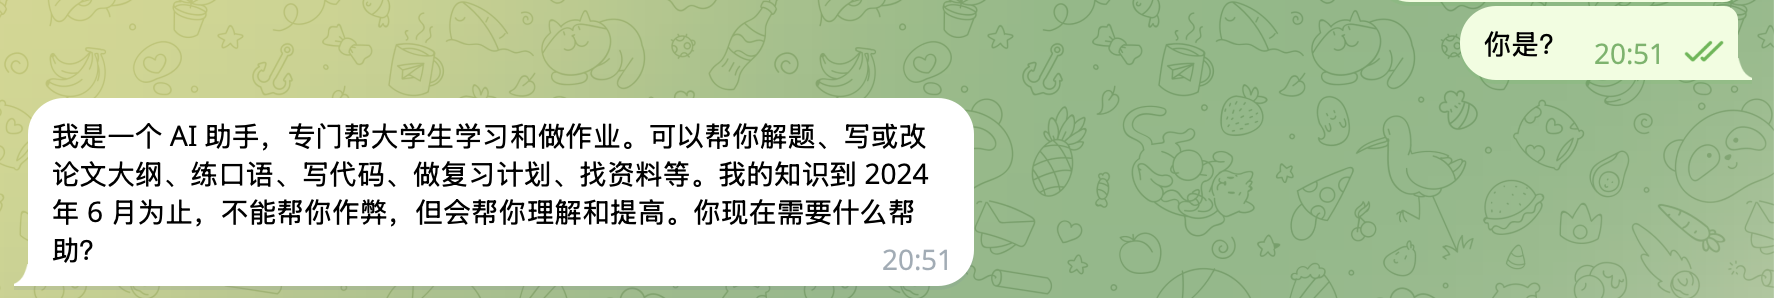
\includegraphics[width=0.95\linewidth]{lab3/telegram_screenshot_1.png}
\end{center}
\begin{center}
  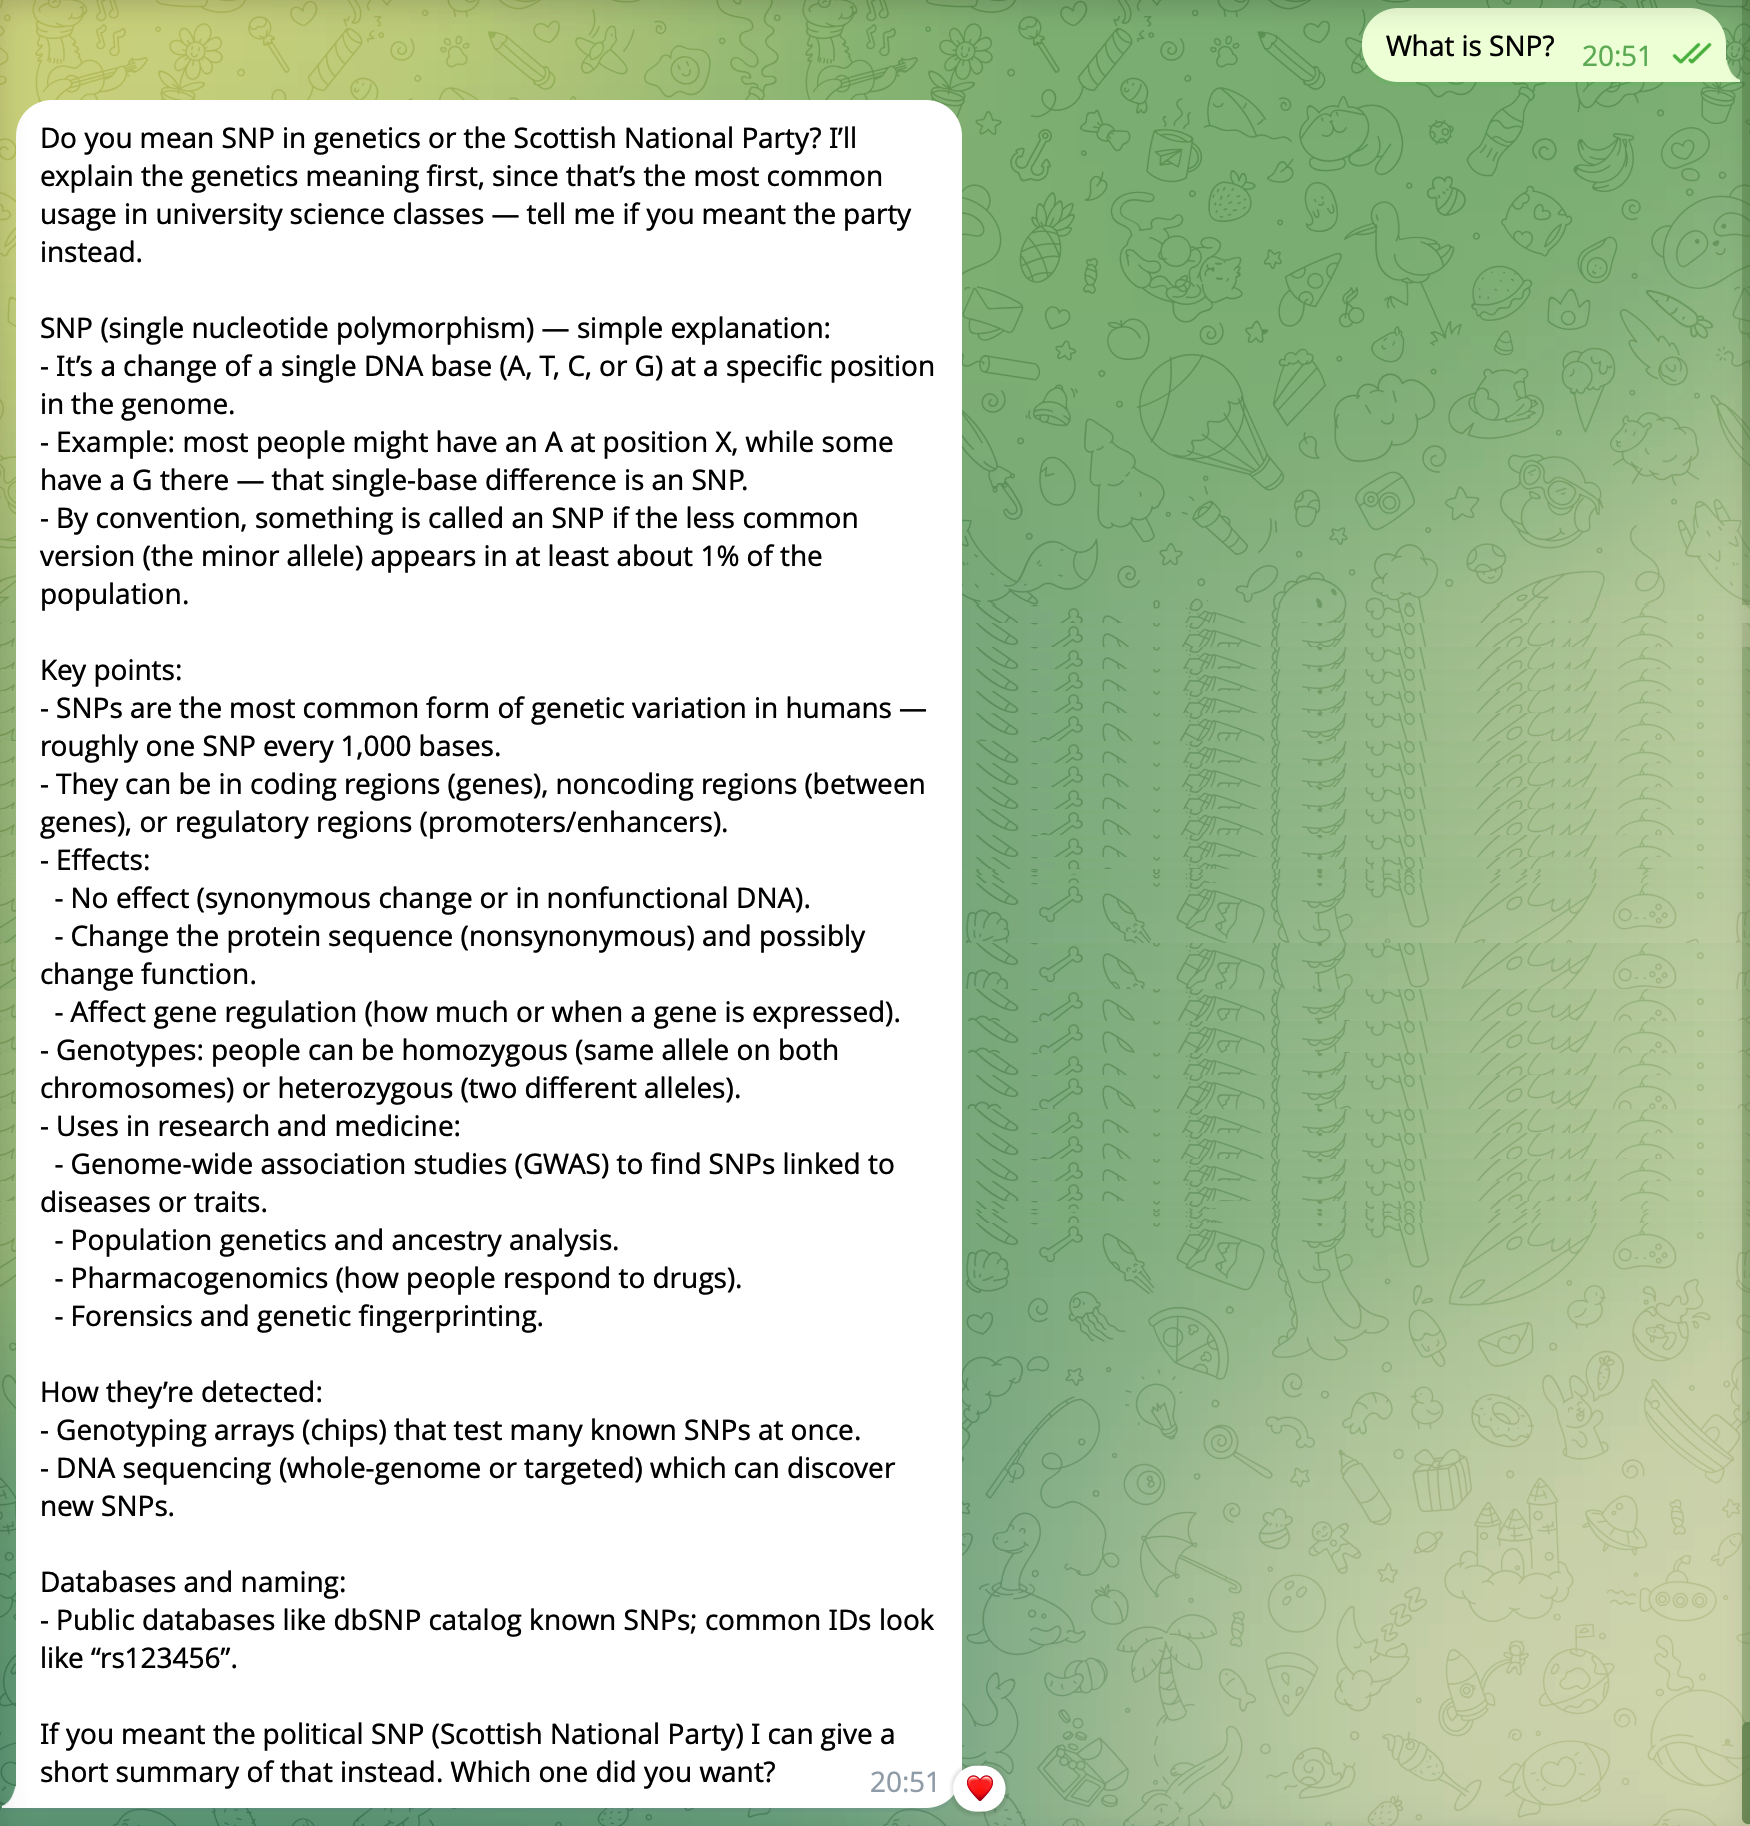
\includegraphics[width=0.95\linewidth]{lab3/telegram_screenshot_2.png}
\end{center}

\section*{3. Terminal Logs}

Here are the logs from running \texttt{python chatbot.py}:
\begin{center}
  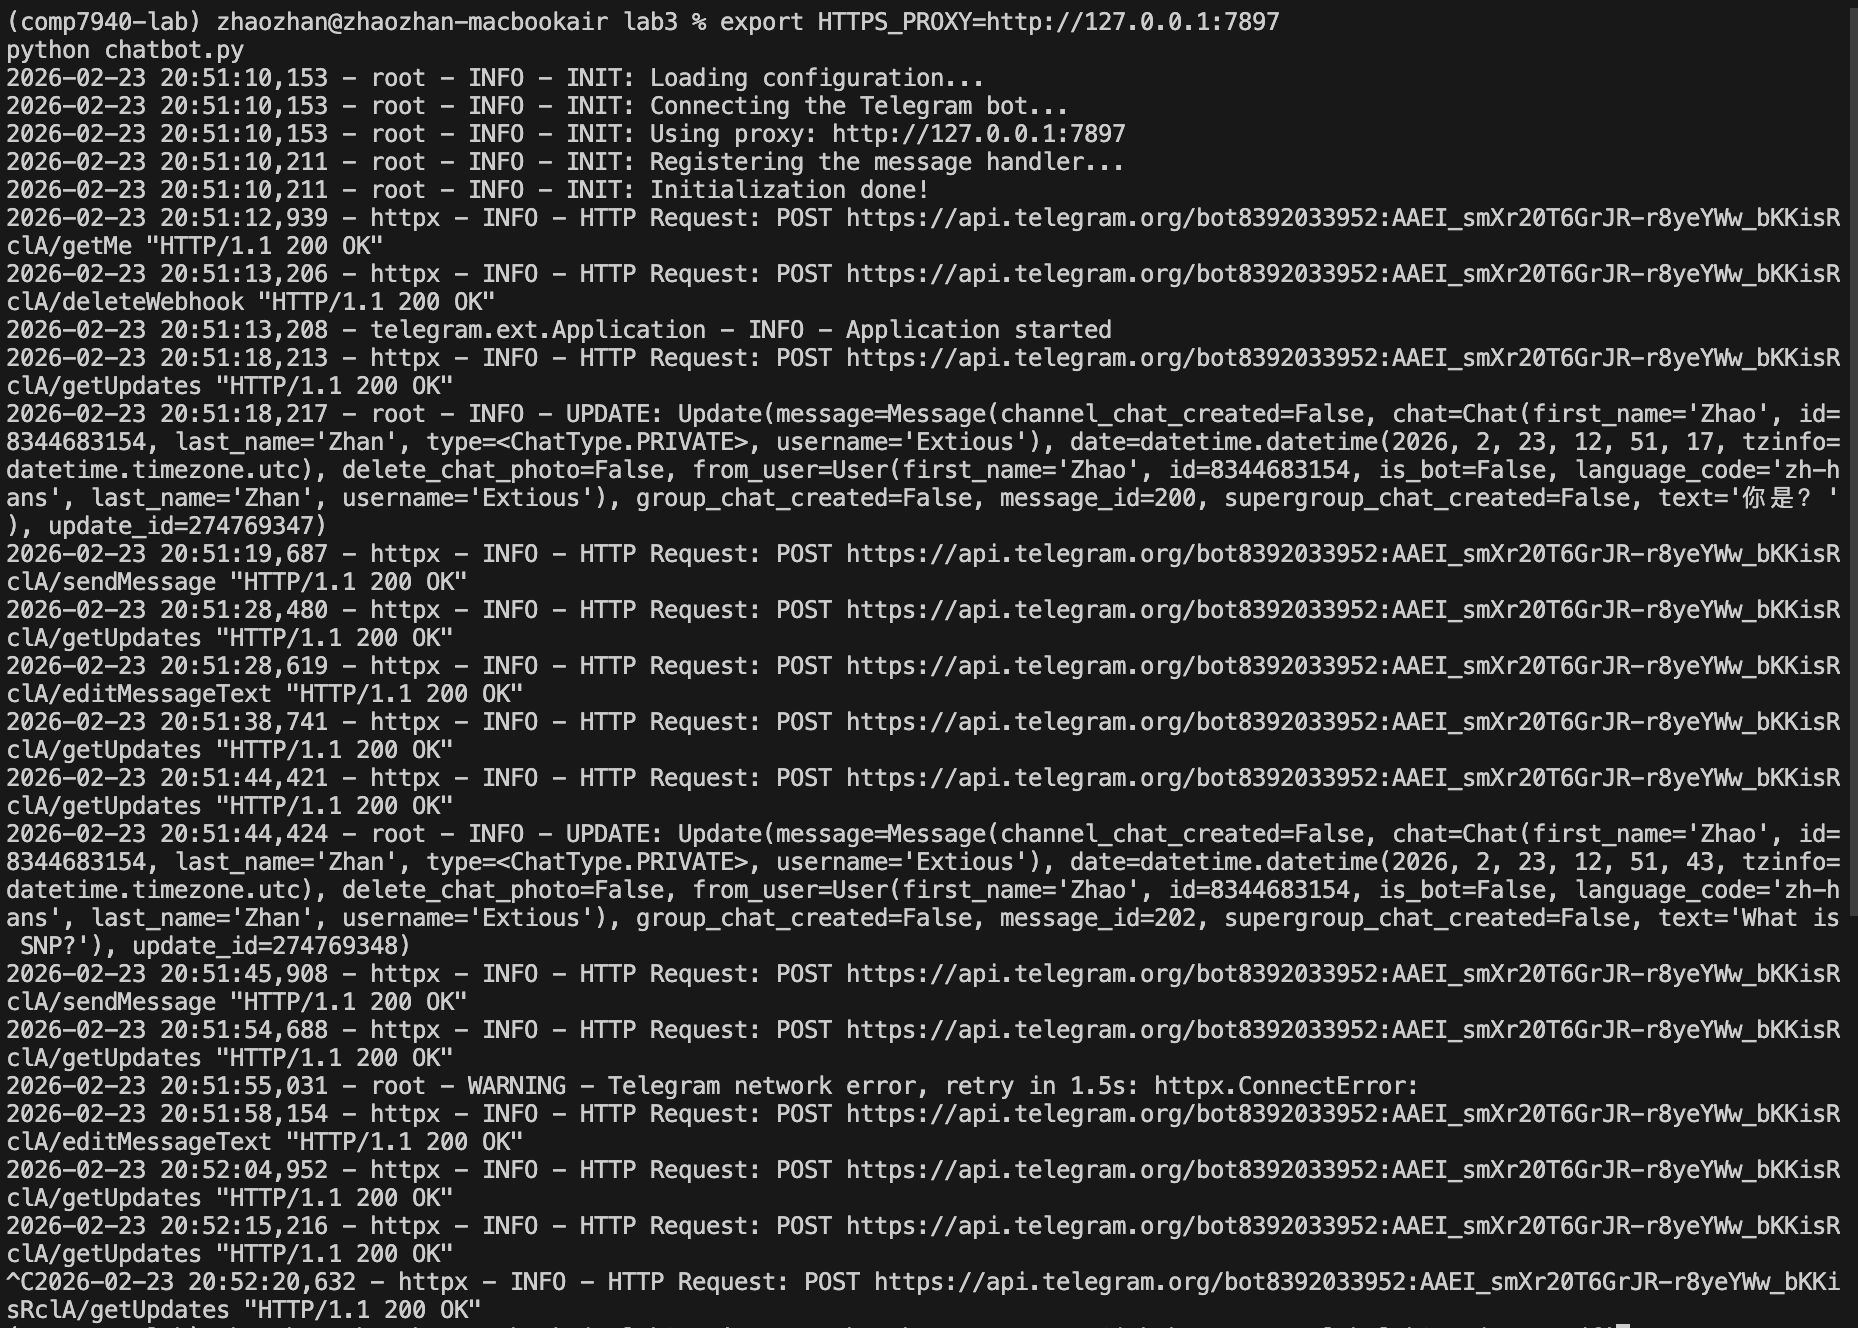
\includegraphics[width=0.95\linewidth]{lab3/logs.png}
\end{center}

\bibliographystyle{plain}
\bibliography{Lab3-25482351-ZHAOZhan}

\end{document}
